\begin{exercise}{2016/17 8}
    Θεωρούμε το σύστημα ελέγχου στο επίπεδο, όπου είναι διαθέσιμα δύο σταθερά
    διανυσματικά πεδία \( X = \frac{\partial}{\partial x} +
    2\frac{\partial}{\partial y} \) και \( Y = 2\frac{\partial}{\partial x}
    + \frac{\partial}{\partial y} \) και επιτρέπεται να προχωρούμε με το ένα ή
    το άλλο διανυσματικό πεδίο, ή με τα αντίστροφά τους, δηλαδή μόνο με τις ροές
    \( \phi^X \) και \( \phi^Y \) των \( X \) και \( Y \).
    \begin{enumerate}[label= (\alph*)]
        \item Δείξτε ότι το \emph{προσβάσιμο σύνολο} \( \mathcal{R}(\vc{0}, T)
            \) των σημείων που μπορούμε να φτάσουμε σε χρόνο \( \leq T \) από το
            αρχικό σημείο \( \vc{0} \) είναι το \( \{x\in\mathbb{R}^2: \|Bx\|_1
            \leq c \} \), όπου \( \|x\|_1 = |x| + |y| \) είναι η \(1-\)νόρμα και
            \( B \) κατάλληλος \( 2 \times 2 \) πίνακας. Βρείτε τον \( B \) και
            τη σταθερά \( c \).
        \item Εάν τώρα περιορίσουμε το χώρο κατάστασης στο κλειστό τετράγωνο με
            κέντρο το \( \vc{0} \) και πλάτος \( 2 \) (δεν επιτρέπεται να βγούμε
            από αυτόν), δείξτε ότι κάθε σημείο του εσωτερικού του είναι
            προσβάσιμο, αλλά για κάποια σημεία στο σύνορο, δεν μπορούμε να
            φτάσουμε με πεπερασμένο αριθμό αλλαγών ροής. Ποια είναι τα σημεία
            αυτά;
    \end{enumerate}
\end{exercise}
\begin{solution}
    (α). Το διανυσματικό πεδίο \( X \) αντιστοιχεί στις διαφορικές εξισώσεις
    \[
        \dot{x} = 1, \quad \dot{y} = 2,
    \]
    που μας δίνει τις λύσεις
    \[
        x = t + x_0, \quad y = t + y_0.
    \]
    Αυτό σε μορφή ροής μπορεί να γραφτεί
    \[
        \phi^X_t(x_0, y_0) = (t + x_0, 2t + y_0),
    \]
    ή πιο γενικά χωρίς το δείκτη με το μηδέν
    \[
        \phi^X_t(x, y) = (t + x, 2t + y), \quad t \in \mathbb{R}.
    \]
    Αντίστοιχα για το διανυσματικό πεδίο \( Y \) προκύπτει η ροή
    \[
        \phi^Y_t(x, y) = (2t + x, t + y), \quad t \in \mathbb{R}.
    \]

    Παρατηρούμε ότι το να κινηθούμε πίσω στο χρόνο είναι το ίδιο με το να
    κινηθούμε μπροστά στο χρόνο με το αντίθετο διανυσματικό πεδίο. Επίσης,
    επειδή τα πεδία είναι γραμμικά και σταθερά η σειρά με την οποία θα κινηθούμε
    δεν παίζει ρόλο. Αυτό που παίζει ρόλο είναι για πόσο χρόνο θα κινηθούμε με το
    κάθε πεδίο. Για παράδειγμα, το να κινηθούμε με την ροή του \( Y \) για χρόνο
    \( c \), μετά με την ροή του \( X \) για χρόνο \( b \) και τέλος με την
    ροή του \( Y \) για χρόνο \( a \), είναι το ίδιο με το να κινηθούμε με την
    ροή του \( X \) για χρόνο \( b \), μετά με την ροή του \( Y \) για χρόνο
    \( c \) και τέλος με την ροή του \( Y \) για χρόνο \( a \). Δηλαδή
    ισχύει
    \[
        \phi^Y_{c} \circ \phi^X_{b} \circ \phi^Y_{a} =
        \phi^X_{b} \circ \phi^Y_{c} \circ \phi^Y_{a}.
    \]

    Ορίζουμε τα χρονικά διαστήματα που κινηθήκαμε συνολικά με την κάθε ροή.
    Έτσι συμβολίζουμε με \( t_x \in \mathbb{R} \) το συνολικό χρόνο που
    κινηθήκαμε με τη ροή του \( X \), δηλαδή την \( \phi^{X}_{t_x} \).
    Αντίστοιχα, με \( t_y \in \mathbb{R} \) το συνολικό χρόνο που κινηθήκαμε
    με τη ροή του \( Y \), δηλαδή την \( \phi^{Y}_{t_y} \).

    Το προσβάσιμο σύνολο είναι η σύνθεση όλων των δυνατών συνδυασμών των ροών.
    Όμως διότι στην περίπτωση αυτή, δεν παίζει ρόλο ο τρόπος με των οποίο θα
    κινηθούμε αλλά μόνο ο συνολικός χρόνος παραμονής στην κάθε ροή, έτσι έχουμε
    ότι το προσβάσιμο σύνολο είναι
    \begin{align}\label{eq:ex8_flow}
        \phi^X_{t_x} \circ \phi^Y_{t_y} (x, y) &=
        \phi^X_{t_x} (2t_y + x, t_x + y) \nonumber \\
        &= (t_x + 2t_y + x, 2t_x + t_y + y).
    \end{align}
    Η παραπάνω σχέση δέχεται σαν είσοδο κάποια \( (x, y) \in \mathbb{R}^2 \) και
    δίνει σαν έξοδο το παραπάνω διάνυσμα. Οπότε είναι ισοδύναμη σχέση με τη
    σύνολο της εκφώνησης. Αν πάρουμε την \(1-\)νόρμα για το αρχικό σημείο
    \( (0, 0) \) προκύπτει
    \[
        |t_x + 2t_y| + |2t_x + t_y| \leq |t_x| + 2|t_y|  + 2|t_x| + |t_y|,
    \]
    όπου το δεύτερο μέλος της ανισότητας ισούται
    \[
        3|t_x| + 3|t_y| = 3(|t_x| + |t_y|) = 3T,
    \]
    όπου \( T \) είναι η συνολική χρονική διάρκεια που κινηθήκαμε με τα διανυσματικά πεδία.

    (β).
    Αν τώρα περιορίσουμε το χώρο κατάστασης στον κλειστό τετράγωνο με
    κέντρο το \( 0 \) και πλάτος το \( 2 \) τότε για να φτάσουμε στο σημείο,
    του χώρου κατάστασης, με συντεταγμένες \( (a, b) \) από τη
    σχέση~\eqref{eq:ex8_flow} ισχύει
    \begin{align*}
        t_x + 2t_y &= a \\
        2t_x + t_y &= b.
    \end{align*}
    Λύνοντας τις παραπάνω ως προς \( t_x, t_y \) προκύπτει
    \begin{equation}\label{eq:ex8_tx_ty}
        t_x = \frac{2b - a}{3}, \quad t_y = \frac{2a - b}{3}.
    \end{equation}

    Ξεκινώντας από το \( (0, 0) \), οι χρόνοι που μπορούμε να κινηθούμε
    με τις ροές των διανυσματικών πεδίων \( X \) και \( Y \) περιορίζονται από
    τις σχέσεις
    \begin{equation}\label{eq:ex8_limits}
        -0.5 \leq t_x \leq 0.5
        \quad \text{\gr{και}} \quad
        -0.5 \leq t_y \leq 0.5,
    \end{equation}
    καθώς διαφορετικά θα βγούμε εκτός των επιτρεπόμενων ορίων. Επομένως για το
    χρόνο \( t_x \) ισχύει
    \begin{align}\label{eq:ex8_b_lim1}
        &-0.5 \leq t_x \leq 0.5 \nonumber \\
        &-0.5 \leq \frac{2b - a}{3} \leq 0.5 \nonumber \\
        &\frac{1}{2}a - \frac{3}{4} \leq b \leq \frac{1}{2}a + \frac{3}{4}.
    \end{align}
    Αντίστοιχα για το χρόνο \( t_y \) ισχύει
    \begin{align}\label{eq:ex8_b_lim2}
        &-0.5 \leq t_y \leq 0.5 \nonumber \\
        &-0.5 \leq \frac{2a - b}{3} \leq 0.5 \nonumber \\
        &2a - \frac{3}{2} \leq b \leq 2a + \frac{3}{2}.
    \end{align}

    Οι ανισώσεις~\eqref{eq:ex8_b_lim1} και~\eqref{eq:ex8_b_lim2} καθώς και τα
    προφανή όρια \( -1 \leq a \leq 1 \) και \( -1 \leq b \leq 1 \) ορίζουν το
    προσβάσιμο σύνολο με μία αλλαγή ροής, δηλαδή από τη ροή \( X \) στη \( Y \) ή
    αντίστροφα. Το σύνολο αυτό απεικονίζεται στο σχήμα~\ref{fig:ex8_rhombus1}.
    Η πορτοκαλί διακεκομμένη γραμμή και το εσωτερικό αυτής, δείχνουν το σύνολο των σημείων
    που είναι προσβάσιμα με μία μονάχα αλλαγή ροής και φυσικά παραμένοντας εντός
    των ορίων που ορίζουν οι σχέσεις~\eqref{eq:ex8_limits}.
    \begin{figure}[h]
        \centering
        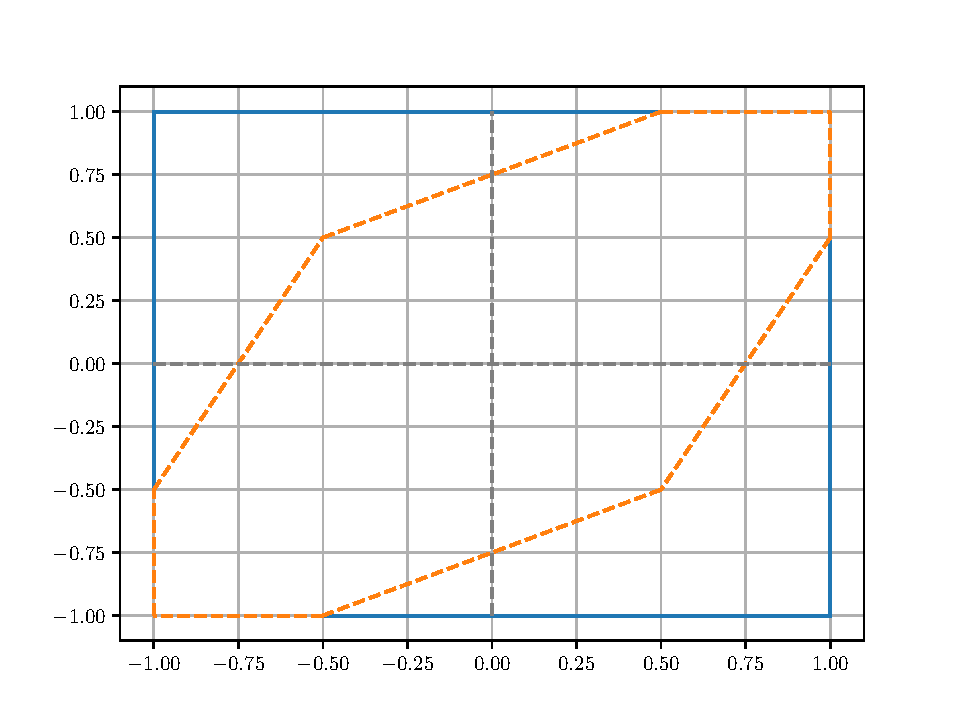
\includegraphics[width=0.9\textwidth]{figures/ex8_rhombus1.pdf}
        \caption{\gr{Προσβάσιμο σύνολο με μία αλλαγή ροής}}
        \label{fig:ex8_rhombus1}
    \end{figure}

    Άρα για να καλύψουμε το υπόλοιπο τετράγωνο, μπορούμε να κινηθούμε σε κάποιο
    σημείο εντός του πορτοκαλί \enquote*{ρόμβου} και θεωρώντας το σημείο αυτό ως
    αρχικό να επαναλάβουμε την ίδια διαδικασία. Έτσι θα δημιουργήσουμε έναν
    μικρότερο \enquote*{ρόμβο} και τελικά θα καλύψουμε όλο το τετράγωνο.
    \begin{figure}[h]
        \centering
        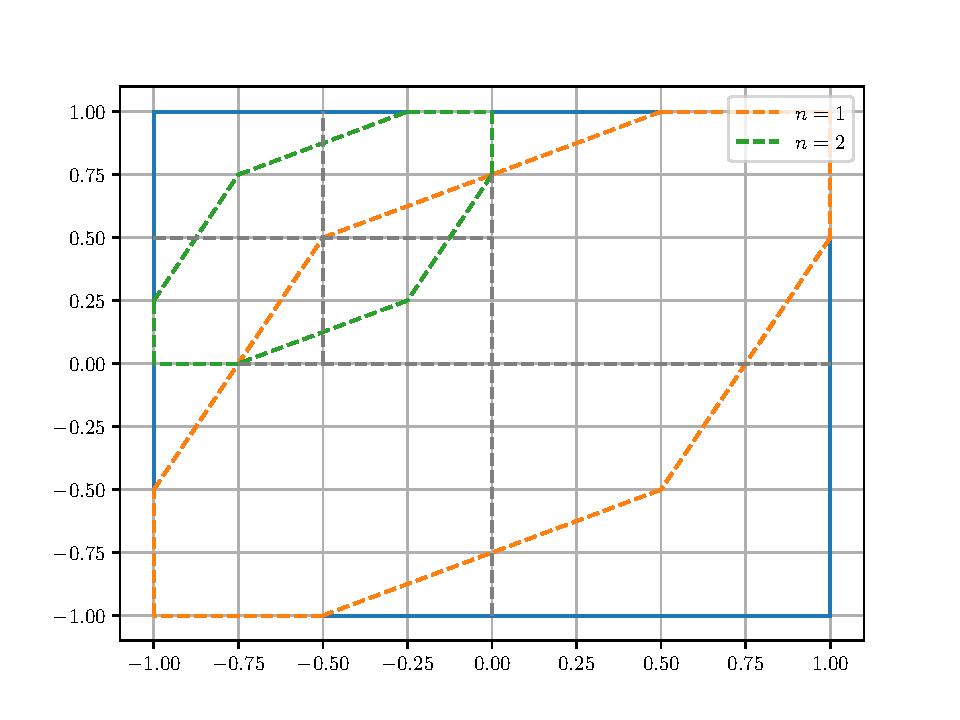
\includegraphics[width=0.9\textwidth]{figures/ex8_rhombus2.pdf}
        \caption{\gr{Προσβάσιμο σύνολο με δύο αλλαγές ροής}}
        \label{fig:ex8_rhombus2}
    \end{figure}
    Για παράδειγμα στο σχήμα~\ref{fig:ex8_rhombus2} εφαρμόσαμε το πεδίο \( X \)
    για χρόνο \( t_x = 0.5 \), μετά το πεδίο \( Y \) για χρόνο \( t_y = -0.5 \)
    και φτάσαμε στο σημείο \( (a, b) = (-0.5, 0.5) \). Από το σημείο αυτό
    εφαρμόζουμε την ίδια ακριβώς διαδικασία που κάναμε παραπάνω. Έτσι με μία
    αλλαγή ροής, δηλαδή από τη ροή \( X \) στη \( Y \) ή αντίστροφα, μπορούμε να
    φτάσουμε όλα τα σημεία που είναι στην πράσινη διακεκομμένη γραμμή και εντός
    αυτής.

    Λόγω της κίνησης που ορίζουν τα διανυσματικά πεδία, ο τρόπος για να φτάσουμε
    οποιοδήποτε σημείο του επάνω δεξιά τεταρτημορίου είναι ακριβώς ο αντίθετος
    για να φτάσουμε οποιοδήποτε σημείο του κάτω αριστερά τεταρτημόριου.
    Αντίστοιχα, το ίδιο ισχύει για το επάνω αριστερά και κάτω δεξιά
    τεταρτημόριο.

    Θα περιγράψουμε έναν τρόπο για να καλύψουμε τα σημεία του επάνω
    δεξιά τεταρτημορίου. Κοιτώντας το σχήμα~\ref{fig:ex8_rhombus1} βλέπουμε ότι
    η ροή, πορτοκαλί διακεκομμένη γραμμή, καλύπτει σχεδόν όλο το τεταρτημόριο
    εκτός από δύο τρίγωνα. Για να καλύψει κάποιος το επάνω τρίγωνο μπορεί να
    κινηθεί με τα εξής βήματα. Μεταφέρεται στο σημείο \( (0, 0.5) \). Θεωρώντας
    το τετράγωνο με κέντρο το σημείο αυτό και πλάτος \( 1 \), θα δημιουργηθεί
    προσβάσιμο σύνολο ανάλογο με αυτό που φαίνεται στο
    σχήμα~\ref{fig:ex8_rhombus2} με την πράσινη γραμμή, με την επάνω παράλληλη
    γραμμή του \enquote*{ρόμβου} να είναι στο επίπεδο \( y = 1 \) και από \( x =
    0.25 \) μέχρι \( x = 0.5 \). Με ακριβώς τον ίδιο τρόπο αν θεωρήσουμε το
    τετράγωνο με κέντρο το \( (-0.25, 0.5) \), η επάνω παράλληλη γραμμή του
    \enquote*{ρόμβου} θα είναι στο επίπεδο \( y = 1 \) και από \( x =
    0 \) μέχρι \( x = 0.25 \). Έτσι θα έχουμε καλύψει το επάνω τρίγωνο. Ομοίως
    θεωρώντας τα τετράγωνα με κέντρα τα σημεία \( (0.5, 0) \) και \( (0.5,
    -0.25) \) και πλάτη \( 1 \), θα καλύψουμε και το άλλο τρίγωνο και συνεπώς
    θα έχουμε καλύψει όλο το επάνω δεξιά τεταρτημόριο. Όπως αναφέραμε,
    ακολουθώντας ακριβώς την αντίθετη διαδικασία μπορούμε να καλύψουμε το κάτω
    αριστερά τεταρτημόριο.

    Συνεπώς μένει να περιγράψουμε έναν τρόπο ούτως ώστε να καλύψουμε το επάνω
    αριστερά τεταρτημόριο. Όπως φαίνεται και στο σχήμα~\ref{fig:ex8_rhombus2}
    μπορούμε να μεταφερθούμε στο ακραίο αριστερό σημείο της πορτοκαλής
    διακεκομμένης, δηλαδή στο σημείο \( (-0.5, 0.5) \) και να θεωρήσουμε
    τετράγωνο με κέντρο το σημείο αυτό και πλάτος \( 1 \). Έτσι θα δημιουργηθεί
    το πράσινο προσβάσιμο σύνολο. Ομοίως για να καλύψουμε την επιφάνεια που
    απομένει από το επάνω αριστερά τεταρτημόριο, θα θεωρήσουμε τετράγωνο στο
    αριστερό ακραίο σημείο, δηλαδή στο \( (-0.75, 0.75) \) και πλάτος \( 0.5 \).

    Όπως καταλαβαίνουμε το σημείο \( (-1, 1) \), θα είναι το τελευταίο σημείο του
    συγκεκριμένου τεταρτημορίου που μελετάμε, που μπορούμε να προσεγγίσουμε.
    Σε κάθε βήμα δηλαδή, το ακραίο αριστερό σημείο του εκάστοτε προσβάσιμου συνόλου
    θα απέχει από τη γωνία \( (-1, 1) \) του τετραγώνου. Αν θεωρήσουμε ότι το αρχικό πλάτος
    του τετραγώνου είναι \( w_0 \) τότε για κάθε νέο τετράγωνο που θεωρούμε το πλάτος
    είναι ίσο με το μισό του προηγούμενου. Αυτό εκφράζεται από τη σχέση
    \[
        w_{n} = \frac{w_{n - 1}}{2},
    \]
    και συναρτήσει του αρχικού πλάτους \( w_0 \) η παραπάνω γράφεται
    \[
        w_n = \frac{w_0}{2^n}.
    \]
    Στο \(n-\)οστό βήμα, η απόσταση του ακραίου αριστερού σημείου του
    \(n-\)οστού προσβάσιμου συνόλου θα απέχει από τη γωνία \( (-1, 1) \) του
    τετραγώνου
    \[
        \left(\frac{w_n}{4}\right)^2 + \left(\frac{w_n}{4}\right)^2
        = \frac{w_n^2}{16} = \frac{w_n^2}{2^4}.
    \]
    Η παραπάνω απόσταση συναρτήσει του αρχικού πλάτος \( w_0 \) γράφεται
    \[
        \frac{w_n^2}{2^4} = \frac{\left(\frac{w_0}{2^n}\right)^2}{2^4}
        = \frac{w_0^2}{2^{2n + 4}}.
    \]
    Καθώς το \( n \to \infty \) η παραπάνω τείνει στο μηδέν. Συνεπώς για
    μη-πεπερασμένο αριθμό αλλαγών ροής η απόσταση θα μηδενιστεί και θα έχουμε
    καλύψει πλήρως κάθε σημείο του επάνω αριστερά τεταρτημορίου. Με αντίθετη διαδικασία,
    και με μη-πεπερασμένο αριθμό αλλαγών ροής θα φτάσουμε το ακραίο σημείο
    \( (1, -1) \) και έτσι θα έχουμε καλύψει πλήρως το κάτω δεξιά τεταρτημόριο.

    Τελικά συνδυάζοντας ό,τι περιγράψαμε θα καλύψουμε και τα τέσσερα
    τεταρτημόρια και συνεπώς όλο το κλειστό τετράγωνο.
\end{solution}
